\documentclass[12pt, a4paper]{article}
\usepackage[T2A]{fontenc}
\usepackage[utf8]{inputenc}
\usepackage[english,ukrainian]{babel}
\usepackage{amsmath, amssymb}
\usepackage{verbatim}
\usepackage{minted}
\usepackage{euler}

\usepackage[top = 1.5 cm, left = .75 cm, right = .75 cm, bottom = 1.5 cm]{geometry}
\usepackage[unicode = true, colorlinks = true, linktoc = all, linkcolor = blue]{hyperref}
\usepackage{subcaption}

\usepackage{float}
\usepackage{graphicx}

\usepackage{amsthm}
\newtheorem{lemma}{Лема}
\newtheorem*{lemma*}{Лема}
\newtheorem{theorem}{Теорема}
\newtheorem*{theorem*}{Теорема}
\newtheorem{definition}{Визначення}
\newtheorem*{definition*}{Визначення}
\theoremstyle{definition}
\newtheorem{remark}{Зауваження}
\newtheorem*{remark*}{Зауваження}
\newtheorem{example}{Приклад}
\newtheorem*{example*}{Приклад}
\newtheorem{problem}{Задача}
\newtheorem*{problem*}{Задача}
\newtheorem{solution}{Розв'язок}
\newtheorem*{solution*}{Розв'язок}
\newtheorem{corollary}{Наслідок}
\newtheorem*{corollary*}{Наслідок}

\newcommand{\NN}{\mathbb{N}}
\newcommand{\RR}{\mathbb{R}}
\newcommand{\CC}{\mathbb{C}}
\newcommand{\HH}{\mathcal{H}}
\newcommand{\Max}{\displaystyle\max\limits}
\newcommand{\Sup}{\displaystyle\sup\limits}
\newcommand{\Sum}{\displaystyle\sum\limits}
\newcommand{\Prod}{\displaystyle\prod\limits}
\newcommand{\Int}{\displaystyle\int\limits}
\newcommand{\Iint}{\displaystyle\iint\limits}
\newcommand{\Lim}{\displaystyle\lim\limits}

\newcommand*\diff{\mathop{}\!\mathrm{d}}

\newcommand{\degrees}{^\circ}

\renewcommand{\bf}[1]{\textbf{#1}}
\renewcommand{\epsilon}{\varepsilon}
\renewcommand{\phi}{\varphi}

\newcommand{\ol}[1]{\overline{#1}}
\newcommand{\ul}[1]{\underline{#1}}

\DeclareMathOperator{\signum}{sign}
\DeclareMathOperator{\diam}{diam}
\DeclareMathOperator{\rang}{rang}
\DeclareMathOperator{\const}{const}
\DeclareMathOperator{\cond}{cond}
\DeclareMathOperator{\diagonal}{diag}

\DeclareMathOperator*{\Min}{min}

\setlength\parindent{0pt}
\allowdisplaybreaks

\newcommand{\cover}[2]{
\begin{center}
\hfill \break
  М{\footnotesizeІНІСТЕРСТВО ОСВІТИ ТА НАУКИ} У{\footnotesizeКРАЇНИ} \\
  К{\footnotesizeИЇВСЬКИЙ НАЦІОНАЛЬНИЙ УНІВЕРСИТЕТ ІМЕНІ} Т{\footnotesizeАРАСА} Ш{\footnotesizeЕВЧЕНКА} \\ 
  Ф{\footnotesizeАКУЛЬТЕТ КОМП'ЮТЕРНИХ НАУК ТА КІБЕРНЕТИКИ} \\
  К{\footnotesizeАФЕДРА ОБЧИСЛЮВАЛЬНОЇ МАТЕМАТИКИ}
\end{center}

\vfill 

\begin{center}
  \large{
    Звіт до лабораторної роботи №{#1} на тему: \\ 
    \guillemotleft{}{#2}\guillemotright{}
  }
\end{center}

\vfill 

\begin{flushright}
  Виконав студент групи ОМ-4 \\
  Скибицький Нікіта
\end{flushright}

\vfill 

\begin{center}
    Київ, 2019
\end{center}

\thispagestyle{empty} 
\newpage
}

\newenvironment{system}{%
  \begin{equation}%
    \left\{%
      \begin{aligned}%
}{%
      \end{aligned}%
    \right.%
  \end{equation}%
}
\newenvironment{system*}{%
  \begin{equation*}%
    \left\{%
      \begin{aligned}%
}{%
      \end{aligned}%
    \right.%
  \end{equation*}%
}

\newcommand{\pluseqq}{{\:\:+\!\!=\:\:}}
.sty}

\newcommand{\range}[2]{\ol{#1..#2}}

\begin{document}

\cover{3}{Чисельне розв'язування рівняння теплопровідності}

\tableofcontents

\section{Постановка задачі}

\subsection{Фізична постановка задачі}

Грудочку~алюмінію сферичної~форми діаметром 20~мм, що має~температуру $0 \degrees \text{C}$ вміщено в~середовище з~температурою $300 \degrees \text{C}$. Визначити~час, який потрібен для~підвищення температури в середині цієї~грудочки до $100 \degrees \text{C}$. \medskip

Фізичні характеристики алюмінію: $\lambda = 220 \frac{\text{Вт}}{\text{м} \cdot K}$, $c = 890 \frac{\text{Дж}}{\text{кг} \cdot K}$, $\rho = 2700 \frac{\text{кг}}{\text{м}^3}$, $\gamma = 300 \frac{\text{Вт}}{\text{м}^2 \cdot K}$.

\subsection{Математична постановка задачі}

\subsection{Загальна математична постановка задачі}

В області $\ol Q_T = \{a \le x \le b, 0 \le t \le T\}$ знайти розв'язок одновимірного нестаціонарного рівняння теплопровідності
\begin{equation}
    \frac{\partial u}{\partial t} = \frac{1}{x^m} \frac{\partial}{\partial x} \left( x^m k(x, t) \frac{\partial u}{\partial x} \right) - q(x, t) u + f(x, t), \quad x \in (a, b), \quad t > 0,
\end{equation}
яке задовольняє початкові умови
\begin{equation}
    u(x, 0) = u_0(x), \quad x \in [a, b]
\end{equation}
і крайові умови
\begin{equation}
    \begin{aligned}
        \alpha_1 k(a, t) \frac{\partial u(a, t)}{\partial x} &= \beta_1 u(a, t) - \mu_1(t); \\
        -\alpha_2 k(b, t) \frac{\partial u(b, t)}{\partial x} &= \beta_2 u(b, t) - \mu_2(t),
    \end{aligned}
\end{equation}
де $k(x, t)$, $q(x, t)$, $f(x, t)$, $u_0(x)$, $\mu_1(t)$, $\mu_2(t)$ --- задані функції; $\alpha_k$, $\beta_k$ ($k=1,2$) --- задані невід'ємні сталі, причому виконуються нерівності $0 < k_0 \le k(x, t)$ ($k_0$ --- деяка стала), $q(x, t) \ge 0$, $\alpha_k^2 + \beta_k^2 \ne 0$ ($k=1,2$).

\subsection{Математична постановка задачі варіанту}

В області $\ol Q_T = \{0 \le x \le R, 0 \le t \le T\}$ знайти розв'язок одновимірного рівняння теплопровідності
\begin{equation}
    c \rho \frac{\partial u}{\partial t} = \frac{\lambda}{x^2} \frac{\partial}{\partial x} \left( x^2 \frac{\partial u}{\partial x} \right), \quad x \in (0, R), \quad t > 0,
\end{equation}
яке задовольняє початкові умови
\begin{equation}
    u(x, 0) = u_0(x), \quad x \in [0, R]
\end{equation}
і крайові умови
\begin{equation}
    \begin{aligned}
        \frac{\partial u(0, t)}{\partial x} &= 0; \\
        -\lambda \frac{\partial u(R, t)}{\partial x} &= \gamma ( u(R, t) - u_\text{env} ).
    \end{aligned}
\end{equation}

\section{Аналітичні маніпуляції}

\subsection{Перехід до системи СІ}

$R = 0.01 \text{м}$, $u_0 = 273 \degrees \text{K}$, $u_{\text{env}} = 573 \degrees {K}$, $\lambda = 220 \frac{\text{Вт}}{\text{м} \cdot K}$, $c = 890 \frac{\text{Дж}}{\text{кг} \cdot K}$, $\rho = 2700 \frac{\text{кг}}{\text{м}^3}$, $\gamma = 300 \frac{\text{Вт}}{\text{м}^2 \cdot K}$.

\subsection{Безрозмірні змінні}

Ведемо безрозмірні змінні
\begin{equation}
    v(x, t) = \frac{u(x, t) - u_0}{u_{\text{env}} - u_0}, \qquad t_1 = \frac{a^2 t}{R^2}, \qquad x_1 = \frac{x}{R},
\end{equation}
де $a^2 = \frac{\lambda}{c \rho}$. Отримаємо наступну задачу: в області $\ol Q_T = \{0 \le x_1 \le 1, 0 \le t_1 \le T_1\}$ знайти розв'язок одновимірного рівняння теплопровідності
\begin{equation}
    \frac{\partial v}{\partial t_1} = \frac{1}{x_1^2} \frac{\partial }{\partial x_1} \left( x_1^2 \frac{\partial v}{\partial x_1} \right), \quad x \in (0, 1), \quad t > 0,
\end{equation}
яке задовольняє початкові умови
\begin{equation}
    v(x_1, 0) = 0, \quad x_1 \in [0, 1]
\end{equation}
і крайові умови
\begin{equation}
    \begin{aligned}
        \frac{\partial v(0, t_1)}{\partial x_1} &= 0; \\
        -\frac{\partial v(1, t_1)}{\partial x_1} &= \gamma_1 v(1, t) - \gamma_1,
    \end{aligned}
\end{equation}
де $\gamma_1 = \frac{\gamma R}{\lambda}$.

\subsection{Зауваження}

Формули переходу назад до розмірних змінних (використовуються для побудови графіків):
\begin{equation}
    u(x, t) = v(x, t) \cdot (u_{\text{env}} - u_0) + u_0, \qquad t = \frac{R^2 t_1}{a^2}, \qquad x = x_1 \cdot R.
\end{equation}

Перша крайова умова випливає з міркувань симетрії і введена для забезпечення умови регулярності розв'язку:
\begin{equation}
    x_1^2 \cdot \left| \frac{\partial v(0, t_1)}{\partial x_1} \right| < \infty.
\end{equation}

\section{Теоретичні відомості}

\subsection{Власне різницева схема}

Розглянемо різницеві методи розв'язування останньої задачі. В області $\ol Q_T$ введемо сітку $\ol \omega_{h, \tau} = \ol \omega_h \times \ol \omega_\tau$, де $\ol \omega_h = \{x_i = i h, h = 1/N, i = \range{0}{N}\}$; $\ol \omega_\tau = \{t_j = j \tau, \tau = T/M, j = \range{0}{M}\}$. Позначимо $y_i^j = y(x_i, t_j)$. \medskip

За допомогою інтегро-інтерполяційного методу апроксимуємо нашу задачу різницевою схемою з ваговими коефіцієнтами:
\begin{equation}
    \ol x_i^2 y_{t, i}^j = \sigma \left( \ol p y_x^{j + 1} \right)_{x, i} + (1 - \sigma) \left( \ol p y_x^j \right)_{x, i}, \quad i = \range{1}{N - 1}, \quad j = \range{1}{M},
\end{equation}
з початковими умовами
\begin{equation*}
    y_i^0 = v_0(x_i), \quad i = \range{0}{N},
\end{equation*}
та крайовими умовами
\begin{equation}
    \sigma \ol p_1 y_{\ol x, 0}^{j + 1} + (1 - \sigma) \ol p_1 y_{\ol x, 0}^j = \frac{h}{2} \ol x_0^2 y_0^j;
\end{equation}
\begin{equation}
    -\sigma \ol p_N y_{\ol x, N}^{j + 1} - (1 - \sigma) \ol p_N y_{\ol x, N}^j = \sigma x_N^2 \gamma_1 y_N^{j + 1} + (1 - \sigma) \gamma_1 x_N^2 y_N^j - x_N^2 \ol \gamma_1 + \frac{h}{2} \ol x_N^2 y_N^j,
\end{equation}
де
\begin{equation*}
    \ol x_0^2 = \frac{1}{h} \int_0^{x_1} x^2 \diff x; \qquad \ol x_i^2 = \frac{1}{2h} \int_{x_{i - 1}}^{x_{i + 1}} x^2 \diff x, \quad i = \range{1}{N - 1}; \qquad \ol x_N^2 = \frac{1}{h} \int_{x_{N - 1}}^{x_N} x^2 \diff x;
\end{equation*}
\begin{equation*}
    \ol p_i = a \cdot x_{i - 1/2}^2, \quad i = \range{1}{N}.
\end{equation*}

\subsection{Результати щодо збіжності}

Покладаючи $\sigma = 0$, дістаємо явну схему; при $\sigma = 1$ --- схему з випередженням (повністю неявну схему); при $\sigma = 0.5$ --- симетричну схему Кранка---Ніколсона, яка записується на шаблоні з шести вузлів. \medskip

У разі досить гладких вхідних даних отримана різницева схема стійка при $\sigma \ge 0.5$ і має місце рівномірна збіжність її зі швидкістю $O(h^2 + \tau^{m_\sigma})$, де
\begin{equation*}
    m_\sigma = \begin{cases}
        2, & \text{при} \quad \sigma = 0.5; \\
        1, & \text{при} \quad \sigma \ne 0.5.
    \end{cases}
\end{equation*}

\subsection{Тридіагональна СЛАР}

Різницева схема при $\sigma \ne 0$ буде неявною, тому $y^{j + 1}$ знаходиться як розв'язок СЛАР з тридіагональною матрицею, а саме:
\begin{equation}
    \begin{aligned}
        b_0 v_0 + c_0 v_1 &= d_0, \\
        a_i v_{i - 1} + b_i v_i + c_i v_{i + 1} &= d_i, \quad i = \range{1}{N - 1}, \\
        a_N v_{N - 1} + b_N v_N &= d_N, 
    \end{aligned}
\end{equation}
де
% \begin{equation}
%     c_0 = 1; \quad b_0 = -c_0; \quad d_0 = 0;
% \end{equation}
\begin{equation}
    \begin{aligned}
        c_0 &= \frac{\sigma \tau}{h^2} \ol p_1; \quad b_0 = -\frac{1}{2} \ol x_0^2 - c_0; \\
        d_0 &= -\frac{1}{2} \ol x_0^2 y_0^j - \frac{(1 - \sigma) \tau}{h^2} \ol p_1 \left( y_1^j - y_0^j \right);
    \end{aligned}
\end{equation}
а також
\begin{equation}
    \begin{aligned}
        a_i &= \frac{\sigma \tau}{h^2} \ol p_i; \quad c_i = \frac{\sigma \tau}{h^2} \ol p_{i + 1}; \quad b_i = -\ol x_i^2 - (a_i + c_i); \\
        d_i &= -\ol x_i^2 y_i^j - \frac{(1 - \sigma) \tau}{h^2} \left( \ol p_{i + 1} \left( y_{i + 1}^j - y_i^j \right) - \ol p_i \left( y_i^j - y_{i - 1}^j \right) \right), \quad i = \range{1}{N - 1};
    \end{aligned}
\end{equation}
і нарешті
\begin{equation}
    \begin{aligned}
        a_N &= \frac{\sigma \tau}{h^2} \ol p_N; \quad b_N = -\frac{\sigma \tau}{h} \gamma_1 x_N^2 - \frac{1}{2} \ol x_N^2 - a_N; \\
        d_N &= \frac{(1 - \sigma) \tau}{h} \gamma_1 x_N^2 y_N^j - \frac{\tau}{h} \gamma_1 x_N^2 - \frac{1}{2} \ol x_N^m y_N^j + \frac{(1 - \sigma) \tau}{h^2} \ol p_N \left( y_N^j - y_{N - 1}^j \right).
    \end{aligned}
\end{equation}

\section{Чисельне моделювання}

\subsection{Графіки}

\begin{figure}[H]
    \centering
    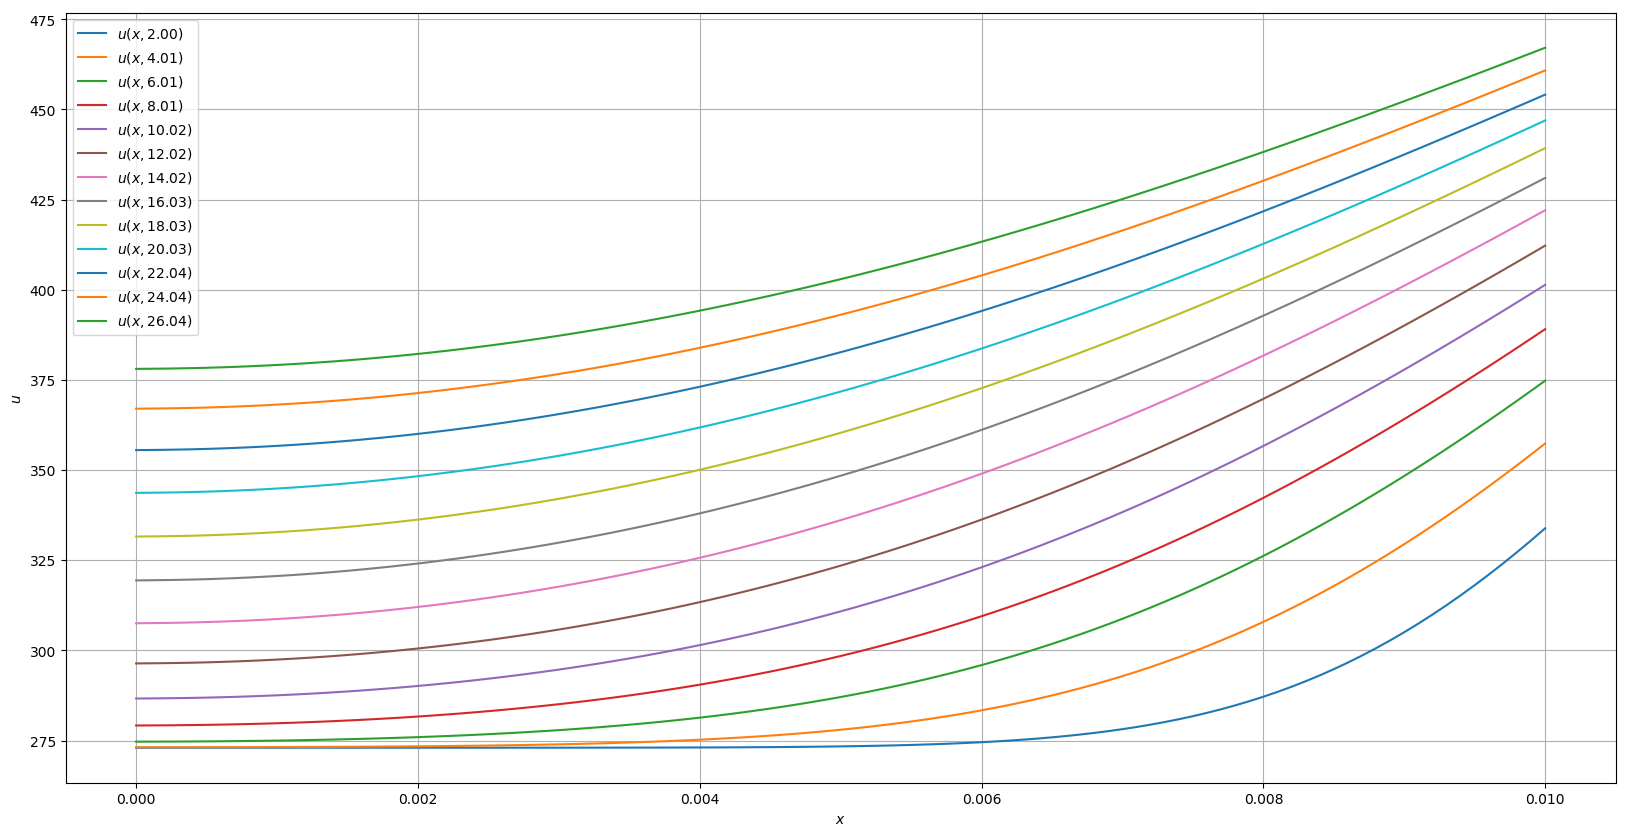
\includegraphics[width=\textwidth]{plots.png}
    \caption{Розподіл температури в залежності від відстані до центру кулі щодві секунди}
\end{figure}

\subsection{Аналіз результатів}

Результат узгоджується із дуже приблизним наближенням: якщо при нагріванні центру до 100 градусів куля у середньому нагріється до 150, то має (з точністю хоча б до порядку) виконуватися наступна рівність:
\begin{equation}
    c \cdot m \cdot (u_{\text{final}} - u_0) = \gamma \cdot t \cdot A_{\text{surface}} \cdot ( u_{\text{env}} - u_{\text{final}} ),
\end{equation}
де $m$ --- маса кулі, $A_{\text{surface}}$ --- площа (eng. \textit{area}) її поверхі; у лівій частині рівності стоїть набута кулею енергія, а у правій --- енергія, передана через границю за час $t$. \medskip

При підстановці $u_{\text{final}} = 150$ знаходимо $t \approx 26.606$. 

\end{document}
